\chapter{Introduction}
The use of unmanned aerial vehicles \acrshort{uav}s in communications is a concept that has been researched in recent years but has not been implemented practically for widespread communications and networking. 
This highlights how recent the concept is of using \acrshort{uav}s in the context of communication networks as an integral part of a network architecture and the need for research to be conducted on this topic for future networks and for specialised applications such as search and rescue operations in regions that are lacking conventional network infrastructure, such as dense urban environments in the wake of natural disasters or remote regions, where it is otherwise not possible to establish a wireless communications network. 

\acrshort{uav}s offer many benefits over conventional, terrestrial network infrastructure in scenarios such as those outlined in this thesis for their ability to be deployed for a critical mission where connectivity must be established rapidly and where the network infrastructure can adapt to the environment. 
Fig. \ref{fig:scope_of_uav_comms} displays the technologies involved in \acrshort{uav} communications and has been adapted from \cite{sharma_communication_2020}. 
Fig. \ref{fig:scope_of_uav_comms} displays the wide range of technologies, enhancements and some applications of \acrshort{uav}-enabled networking, illustrating the many avenues for research into this topic that are being explored. 
This thesis aims to utilise many of these technologies, in particular for communications and networking, while utilising enhancements such as machine learning techniques, physical layer security and optimisation techniques. 

\begin{figure} [ht!]
    \centering
    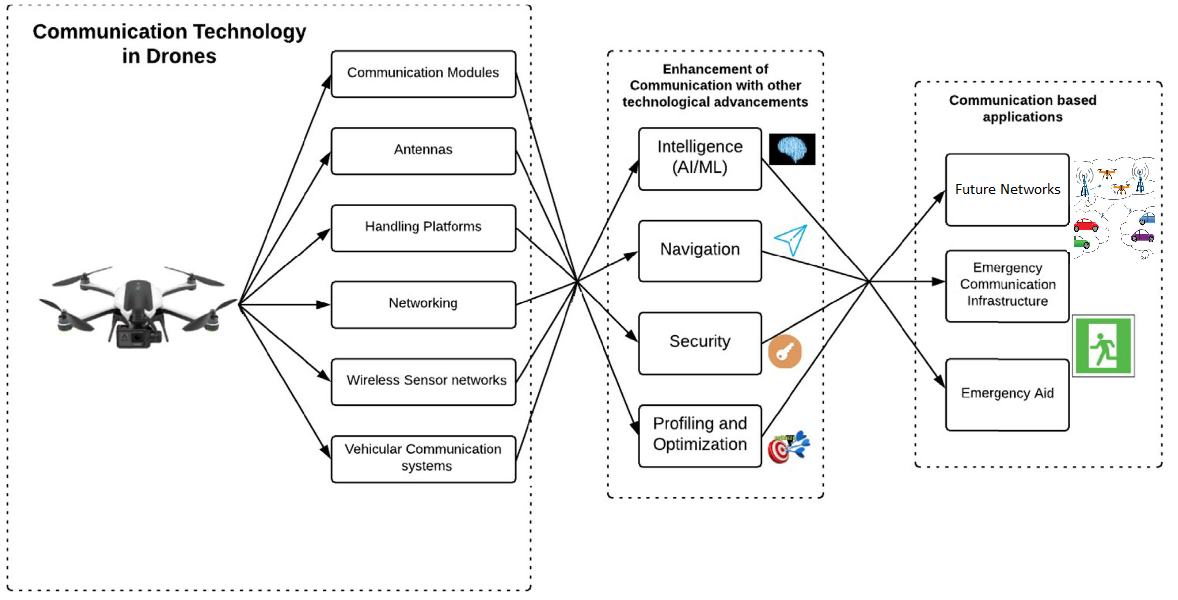
\includegraphics[width=1\linewidth]{figures/edited_scope_of_uav_communications.png}
    \caption{Applications \& Technologies of \acrshort{uav}s for Wireless Communication}
    \label{fig:scope_of_uav_comms}
\end{figure}
\acrshort{uav}s also can enhance the chance of dynamically establishing \acrfull{los} connections with a \acrfull{gu} in ways that are not possible with terrestrial and fixed network infrastructure.
\acrshort{uav}s can be designed and deployed to serve different roles in wireless communications networks, such as acting as a \acrfull{bs} or a relay. 

To ensure efficient use of \acrshort{uav}s as aerial \acrshort{bs}s is achieved, optimisation techniques and deep reinforcement learning (\acrshort{drl}) are employed to model the constraints on the system that are enforced upon an objective function. 
\acrshort{drl} is utilised to enable a \acrshort{uav} to adapt to a range of different scenarios rapidly. 

Simulations applying \acrshort{drl} to this joint optimisation problem have been created using the Python programming language  in which a set of legitimate ground users (\acrshort{gu}s), or legitimate users (\acrshort{lu}s), are provided with network coverage in a physically secure manner with the use of a \acrshort{uav}-\acrshort{bs} while a set of eavesdroppers (referred to as "Eves") who are attempting to conduct \acrfull{mitm} attacks are detecting the \acrshort{uav}-\acrshort{lu} signal that has been spiked with an \acrfull{ans}. 
\acrfull{bash} scripting has been used for running the experiments and handling the storage of the output data from the Python simulations for post-processing and analysis. 
The \acrshort{lu}s are able to filter out the \acrshort{ans}, whereas the Eve is not provided with the \acrshort{ans} information. 

Due to the large volume of data and the large number of highly non-linear relationships between many different aspects of the environment, quantum computing techniques are utilised to offload some of the computation that otherwise would be quite challenging to compute classically. 
This is also done to explore the concept of integrating contemporary quantum computing capabilities into a large and complex joint optimisation problem as this is a very new and developing field of study. 

This thesis aims to solve a joint optimisation problem for \acrshort{uav}-enabled wireless communications and networking with a particular focus on the physical layer security and secrecy of communications for a set of \acrshort{lu}s. 
To solve this joint optimisation problem, many different aspects of the system must be considered and the subproblems to the secrecy rate optimisation problem must also be optimised. 
To do this, the data exchange rate, energy efficiency and \acrshort{uav} trajectory are treated as subproblems to the secrecy rate optimisation problem and they are also optimised. 

As this is an exploration of future networking solutions, \acrfull{5g} and a \acrfull{mimo} system are considered for the wireless communications, with non-orthogonam multiple accessing (\acrshort{noma}) methods being used for the multiple-accessing required for the number of \acrshort{gu}s considered in the simulation environment. 